\documentclass[aspectratio=169]{beamer}

\usetheme[progressbar=frametitle, numbering=fraction]{metropolis}

\usepackage{tikz}
\usetikzlibrary{shapes,arrows,positioning,calc,decorations.pathmorphing}

\usepackage{fontenc}
\usepackage{pdfpc}

% Metadata
\title{From Chords to Code}
\subtitle{Building a Ukulele Companion App}
\author{Baiju Muthukadan}
\institute{Senior Software Engineer, Red Hat}
\date{FOSSMeet 2026 \\ NIT Calicut}

\begin{document}

% ----------------------------------------------------------
% Title Slide
% ----------------------------------------------------------
\begin{frame}
  \begin{columns}
    \column{0.7\textwidth}
      \titlepage
    \column{0.3\textwidth}
      \begin{center}
        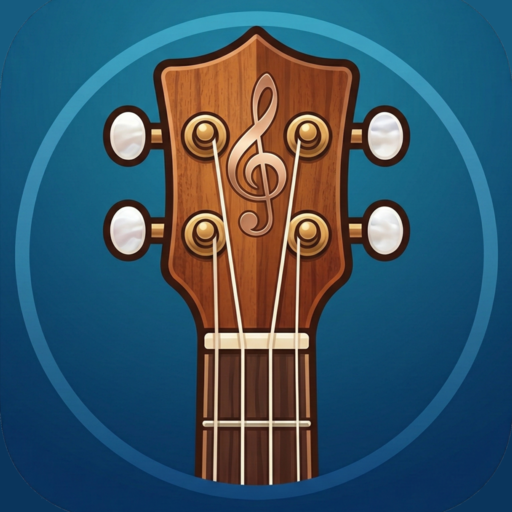
\includegraphics[width=3cm]{app-icon.png}
      \end{center}
  \end{columns}
  \pdfpcnote{Story of how learning a musical instrument led to building and shipping a mobile app -- with AI tools and the open source community.}
\end{frame}

% ----------------------------------------------------------
% Outline
% ----------------------------------------------------------
\begin{frame}{Outline}
  \tableofcontents
  \pdfpcnote{Overview: how it began, idea to app, architecture, shipping challenges, FOSS principles, lessons learned, live demo.}
\end{frame}

% ==========================================================
\section{Introduction}
% ==========================================================

\begin{frame}{About Me}
  \begin{itemize}
    \item 20+ years in software industry
    \item Senior Software Engineer at Red Hat
    \item Active FOSS contributor
    \item Exploring AI in software development
  \end{itemize}
  \pdfpcnote{20+ years in industry. Work at Red Hat. Long-time FOSS contributor. Recently exploring AI in software development -- central theme of this talk.}
\end{frame}

\begin{frame}{The Spark}
  \begin{itemize}
    \item Started learning ukulele --- couldn't find the right app
    \item Was exploring AI-assisted development (Claude Code, Cursor)
    \item ``Why not build one myself?''
    \item Built it for personal use --- not planning to distribute
    \item Shared on Reddit (\texttt{r/ukulele}) --- real interest from the community
    \item Community response turned a side project into a real one!
  \end{itemize}
  \pdfpcnote{Picked up ukulele, looked for apps, none did what I wanted. Was exploring Claude Code and Cursor. Built it for myself. Posted on r/ukulele -- people were genuinely interested. That response changed everything.}
\end{frame}

% ==========================================================
\section{From Idea to App}
% ==========================================================

\begin{frame}{The Problem}
  \begin{itemize}
    \item Plenty of apps show chord diagrams for common chords
    \item But \textit{how} are those chords found on the fretboard?
    \item Wanted a \textbf{fretboard explorer} --- not just a chord dictionary
    \item Press on strings, strum, and see what chord you're playing
    \item Learn the ``why'' behind chord shapes, not just memorize them
  \end{itemize}
  \pdfpcnote{Plenty of chord diagram apps exist. But how are chords found on the fretboard? Wanted to press strings and see the chord. Understand the ``why'' not just memorize positions.}
\end{frame}

\begin{frame}{Early Prototyping}
  \begin{itemize}
    \item Chatted with AI chatbots (ChatGPT, Gemini) to explore app requirements
    \item Used conversations to understand music theory and fretboard logic
    \item AI as a brainstorming partner --- not just a code generator
  \end{itemize}
  \pdfpcnote{Before writing code, chatted with ChatGPT and Gemini. Not for code generation -- for requirements. What should a fretboard explorer do? How does music theory work? AI as brainstorming partner.}
\end{frame}

\begin{frame}{Building with AI Tools}
  \begin{itemize}
    \item Started building features with Cursor and Claude Code
    \item Slowly added functionality --- iterate, test, improve
    \item AI-assisted development, but human-driven decisions
  \end{itemize}
  \pdfpcnote{Used Cursor and Claude Code to build. Very iterative -- build, test, improve. AI helped write code faster, but all decisions about what to build and how were mine.}
\end{frame}

\begin{frame}{From Prototype to Production}
  \begin{itemize}
    \item Had a working app --- now what?
    \item Needed real users to validate and improve it
    \item Google Play requires closed testing before publishing
    \item The next challenge: getting the app out there
  \end{itemize}
  \pdfpcnote{Had a working app on my phone. Now what? Need real users. Google Play requires closed testing before publishing -- much bigger challenge than expected.}
\end{frame}

% ==========================================================
\section{Design \& Architecture}
% ==========================================================

\begin{frame}{The iOS Question}
  \begin{itemize}
    \item Users on Reddit and Facebook kept asking: ``What about iOS?''
    \item Didn't own any Apple device
    \item Purchased an iPad mini to make it happen
    \item Decided to go cross-platform
  \end{itemize}
  \pdfpcnote{On Reddit and Facebook, people kept asking ``What about iOS?'' Didn't own any Apple device. Bought an iPad mini. Decided to go cross-platform.}
\end{frame}

\begin{frame}{Choosing the Tech Stack}
  \begin{itemize}
    \item Kotlin Multiplatform (KMP) for shared logic
    \item Android: Jetpack Compose + Material3
    \item iOS: SwiftUI
    \item Shared module: domain logic, pitch detection, chord data
    \item Platform-specific: UI, audio, storage
  \end{itemize}
  \pdfpcnote{KMP for shared logic -- write once. Android: Compose + Material3. iOS: SwiftUI. Core logic shared, UI/audio/storage are platform-specific.}
\end{frame}

\begin{frame}{App Architecture}
  \begin{center}
    \begin{tikzpicture}[scale=0.95,
      shared/.style={draw, rounded corners=4pt, minimum width=7.5cm, minimum height=2cm,
        align=center, fill=violet!12, draw=violet!60!black, line width=0.8pt},
      platform/.style={draw, rounded corners=4pt, minimum width=3.5cm, minimum height=2.5cm,
        align=left, line width=0.8pt},
      arrow/.style={->, thick, gray!70},
      label/.style={font=\bfseries\small}
    ]
      % Shared module
      \node[shared] (shared) {\textbf{Shared (KMP Module)} \\ {\small Domain logic, data types, pitch detection, chords}};

      % Android
      \node[platform, fill=green!8, draw=green!50!black, below=1.5cm of shared, xshift=-2.3cm] (android)
        {\textbf{Android App} \\ {\scriptsize Compose + Material3} \\ {\scriptsize ViewModel / StateFlow} \\ {\scriptsize SharedPreferences} \\ {\scriptsize SoundPool (OGG)}};

      % iOS
      \node[platform, fill=orange!8, draw=orange!60!black, below=1.5cm of shared, xshift=2.3cm] (ios)
        {\textbf{iOS App} \\ {\scriptsize SwiftUI} \\ {\scriptsize ObservableObject} \\ {\scriptsize UserDefaults} \\ {\scriptsize AVFoundation (WAV)}};

      % Arrows
      \draw[arrow] ([xshift=-1.2cm]shared.south) -- (android.north);
      \draw[arrow] ([xshift=1.2cm]shared.south) -- (ios.north);
    \end{tikzpicture}
  \end{center}
  \pdfpcnote{Shared KMP module at top -- all music theory and chord logic. Android: Compose, StateFlow, SoundPool. iOS: SwiftUI, ObservableObject, AVFoundation. Same logic, native experience.}
\end{frame}

\begin{frame}{UI/UX Decisions}
  \begin{itemize}
    \item Native look and feel on both platforms (Compose + SwiftUI)
    \item Preferred platform-native widgets and patterns
    \item No pixel-perfect matching between Android and iOS
    \item Each platform feels like it belongs there
  \end{itemize}
  \pdfpcnote{Native look and feel on both platforms. Preferred platform-native widgets over pixel-perfect matching. Android feels like Android, iOS feels like iOS.}
\end{frame}

% ==========================================================
\section{Building \& Shipping}
% ==========================================================

\begin{frame}{Development Workflow}
  \begin{itemize}
    \item AI-assisted development with Cursor and Claude Code
    \item Created custom Skills in Cursor to automate repetitive tasks
    \item Examples: release builds, Play Store uploads, translations
    \item Gradually built a library of reusable workflows
    \item Rules for architecture, accessibility, testing conventions
    \item Result: consistent, repeatable process --- even as a solo developer
  \end{itemize}
  \pdfpcnote{Solo dev needs consistency. Custom Cursor Skills for releases, uploads, translations. Rules for architecture and accessibility. Repeatable process -- move fast without breaking things.}
\end{frame}

\begin{frame}{Reaching Out for Testers}
  \begin{itemize}
    \item Posted on Reddit (\texttt{r/ukulele}) --- 3.9K views, 14 comments
    \item Shared in Facebook ukulele groups
    \item Put out a request on WhatsApp status
    \item Messaged ukulele players on Instagram
    \item Finally got 30+ people to join the Google Group
  \end{itemize}
  \pdfpcnote{Google Play needs closed testers. Reddit post: 3.9K views, 14 comments. Facebook groups, WhatsApp status, Instagram DMs. Got 30+ people in the Google Group.}
\end{frame}

\begin{frame}{The 14-Day Challenge}
  \begin{itemize}
    \item Google Play requires 12+ testers for 14 continuous days
    \item Sent emails asking testers to open the app daily
    \item Play Store dashboard told a different story --- most weren't active
    \item A common struggle for indie developers everywhere
  \end{itemize}
  \pdfpcnote{Getting people to join was half the battle. Google needs 12+ testers active for 14 continuous days. Sent emails daily. Dashboard showed most weren't active. Common indie dev struggle.}
\end{frame}

\begin{frame}{App Hive to the Rescue}
  \begin{itemize}
    \item Discovered App Hive --- a community-driven closed testing hub
    \item Developers form ``Hives'' of 14--20 members
    \item You test their apps, they test yours --- mutual help
    \item Proof-of-test system: screenshots, real devices only
    \item After 14 days of continuous testing --- requirement fulfilled!
    \item Finally published on Google Play Store
  \end{itemize}
  \pdfpcnote{App Hive: community-driven testing platform. Hives of 14-20 devs. You test theirs, they test yours. Screenshots required, real devices only. After 14 days -- requirement fulfilled! Published on Play Store.}
\end{frame}

\begin{frame}{User Feedback \& Iteration}
  \begin{itemize}
    \item Early Reddit feedback: ``practical and beneficial'', ``looks useful''
    \item Feature requests from real users (e.g., baritone tuning)
    \item ``Works fine on tablet and smartphone!'' --- first real user review
    \item Opened source code on GitHub to build trust
    \item Each round of feedback shaped the next release
  \end{itemize}
  \pdfpcnote{Encouraging Reddit feedback. Feature requests like baritone tuning. First review: ``Works fine on tablet and smartphone!'' Opened source on GitHub for trust. Feedback shaped each release.}
\end{frame}

% ==========================================================
\section{FOSS \& the App}
% ==========================================================

\begin{frame}{FOSS Principles in Practice}
  \begin{itemize}
    \item Code is MIT Licensed --- fully open source
    \item During development: release early, release often
    \item After production release: monthly release cadence (unless bugs)
    \item Transparent about development process and decisions
  \end{itemize}
  \pdfpcnote{FOSS from the start. MIT licensed. During dev: release early, release often. After production: monthly cadence unless critical bugs. Transparent about every decision.}
\end{frame}

\begin{frame}{Product Decisions That Mattered}
  \begin{itemize}
    \item No ads, no analytics, no telemetry --- ever
    \item Privacy policy is one sentence: ``This app does not collect any data''
    \item Shipped Google Drive sync, then removed it --- local backup only
    \item Offline-first is a feature, not a limitation
  \end{itemize}
  \pdfpcnote{No ads, no analytics, no telemetry -- ever. Privacy policy is one sentence. Shipped Google Drive sync then removed it. Local only. Offline-first is a feature. Users trust what they control.}
\end{frame}

\begin{frame}{Accessibility: Not an Afterthought}
  \begin{itemize}
    \item Designed for blind and visually impaired musicians
    \item TalkBack (Android) + VoiceOver (iOS) on every element
    \item Tuner readings announced in real time via live regions
    \item High-contrast theme + left-handed mode
    \item Breaking accessibility is treated as seriously as breaking functionality
  \end{itemize}
  \pdfpcnote{Designed for blind/visually impaired musicians. TalkBack and VoiceOver on every element. Tuner uses live regions -- screen reader announces notes in real time. High contrast + left-handed mode.}
\end{frame}

\begin{frame}{Community \& Sharing}
  \begin{itemize}
    \item First community bug report --- fixed within 24 hours
    \item Publicly credited the reporter, explained the root cause
    \item One bug report led to new tests and accessibility checks
    \item Proper attribution: ATTRIBUTION.md credits audio samples,
          ML models, and libraries with their licenses
    \item Open discussions on GitHub for anyone to follow along
  \end{itemize}
  \pdfpcnote{First community bug report -- auto-scroll issue. Fixed in 24 hours. Credited reporter, explained root cause publicly. Led to new tests and accessibility checks. ATTRIBUTION.md credits all resources. Open GitHub discussions.}
\end{frame}

% ==========================================================
\section{Lessons Learned}
% ==========================================================

\begin{frame}{What Worked}
  \begin{itemize}
    \item AI as a force multiplier --- chatbots for requirements, Cursor/Claude Code for building
    \item Posting on Reddit early to validate the idea
    \item Going cross-platform with KMP --- shared logic, native UIs
    \item Custom Cursor Skills for repeatable workflows
    \item App Hive for solving the closed testing bottleneck
    \item Being transparent and community-focused from day one
  \end{itemize}
  \pdfpcnote{AI as force multiplier. Reddit for early validation. KMP for cross-platform. Cursor Skills for workflows. App Hive for testing. Transparency and community from day one.}
\end{frame}

\begin{frame}{What I'd Do Differently}
  \begin{itemize}
    \item Learn more music theory before building a music app
    \item Start the iOS port earlier --- plan for cross-platform from day one
    \item Give the Circle of Fifths feature more focus sooner
  \end{itemize}
  \pdfpcnote{Learn more music theory first -- domain knowledge matters. Plan cross-platform from day one instead of retrofitting. Circle of Fifths is key music theory concept -- should have prioritized earlier.}
\end{frame}

% ==========================================================
\section{Demo}
% ==========================================================

\begin{frame}{Live Demo}
  \begin{center}
    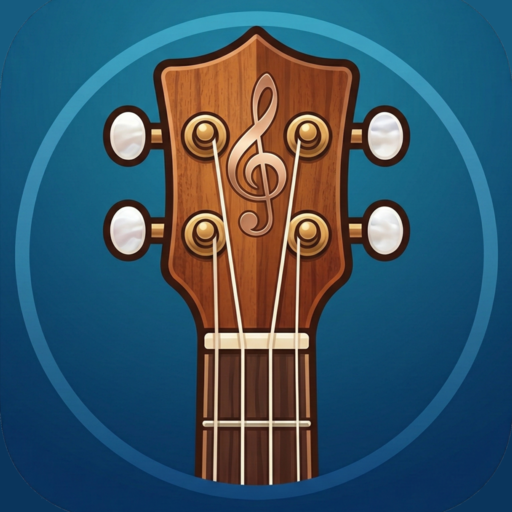
\includegraphics[width=2.5cm]{app-icon.png}

    \vspace{0.5cm}

    {\Large Ukulele Companion App}

    \vspace{0.3cm}

    \textit{Live demo using iOS Simulator}
  \end{center}
  \pdfpcnote{Show fretboard explorer, chord detection, tuner, and songbook. Keep demo under 5 minutes.}
\end{frame}

% ==========================================================
\section{Conclusion}
% ==========================================================

\begin{frame}{The App at a Glance}
  \begin{center}
    \begin{tikzpicture}[
      stat/.style={draw, rounded corners=4pt, minimum width=2.8cm, minimum height=1cm,
        align=center, fill=mDarkTeal!10, draw=mDarkTeal, font=\small\bfseries}
    ]
      \node[stat] (a) at (0,0) {17 features};
      \node[stat] (b) at (3.5,0) {2 platforms};
      \node[stat] (c) at (7,0) {16 languages};
      \node[stat] (d) at (1.75,-1.5) {Fully offline};
      \node[stat] (e) at (5.25,-1.5) {MIT license};
    \end{tikzpicture}
  \end{center}
  \vspace{0.3cm}
  \begin{itemize}
    \item No network, no telemetry, no ads
    \item Available on Google Play and App Store
  \end{itemize}
  \pdfpcnote{Now the numbers: 17 features, 2 platforms, 16 languages, fully offline, MIT licensed. No network, no telemetry, no ads. On both stores.}
\end{frame}

\begin{frame}{Key Takeaways}
  \begin{itemize}
    \item Scratch your own itch --- the best apps solve problems you have yourself
    \item AI tools lower the barrier --- you don't need a team to ship a real product
    \item Share early, listen actively --- Reddit validated the idea before over-investing
    \item FOSS principles build trust --- open source, attribution, transparency
    \item The hardest part isn't code --- it's distribution, testing, and reaching users
    \item Start today --- your side project might surprise you!
  \end{itemize}
  \pdfpcnote{Scratch your own itch. AI lowers the barrier. Share early, listen. FOSS builds trust. Hardest part isn't code -- it's distribution. Start today!}
\end{frame}

\begin{frame}{Get Involved}
  \begin{itemize}
    \item Contributions welcome: features, translations, bug fixes, docs
    \item Available on Google Play and App Store
    \item Companion book: \textit{The Complete Ukulele Learning Book} (free PDF)
    \item \texttt{github.com/baijum/ukulele-companion}
  \end{itemize}
  \pdfpcnote{Contributions welcome: features, translations, bug fixes, docs. On both stores. Free companion book on archive.org. Everything on GitHub.}
\end{frame}

\begin{frame}{Thank You!}
  \begin{center}
    {\Large Questions?}

    \vspace{1cm}

    \texttt{github.com/baijum/ukulele-companion}
  \end{center}
  \pdfpcnote{Thank you! Open for questions. 10 minutes for Q\&A.}
\end{frame}

\end{document}
